% Outline Project Specification Report

%The document is a report
\documentclass[12pt,a4paper]{article}

%define horizontal rule
\newcommand{\HRule}{\rule{\linewidth}{0.5mm}}

\usepackage{fullpage}

%use the listings package
\usepackage{listings}
%use the English language
\usepackage[english]{babel}
%use graphics
\usepackage{graphicx}
%use wrap figures
\usepackage{wrapfig}
%geometry stuffs
\usepackage{lscape}
%use natbib bibliography package
%\usepackage[numbers]{natbib}
%use harvard bibliography package
%\usepackage{harvard}	
%use captions
\usepackage{caption}
%use multi-row tables
\usepackage{multirow}
\usepackage{url}
\usepackage{subcaption}

\begin{document}

%use harvard citations
%\citationstyle{agsm}

%include the title page
\newcommand{\Revision}{678f948}

\begin{titlepage}
 
\begin{center}

% Upper part of the page

\includegraphics[width=0.20\textwidth]{../cover_logo.png}\\[1cm]


\textsc{\LARGE Aberystwyth University}\\[0.5cm]
\textsc{\LARGE Final Report}\\[0.5cm]



 
% Title
\HRule \\[0.4cm]
{ \huge \bfseries Partridge: An Intelligent Literature Analysis and
Recommendation Suite.}\\[0.4cm]

\HRule \\[1.5cm]

 % Author and student ID
\begin{minipage}{0.4\textwidth}
\begin{flushleft} \large
\emph{Author:}\\
\textsc{James Ravenscroft}\\
jrr9@aber.ac.uk\\
090407039\\
\end{flushleft}
\end{minipage}
\begin{minipage}{0.4\textwidth}
\begin{flushright} \large
\emph{Supervisors} \\
Amanda Clare (afc)\\
Maria Liakata (mal)

\end{flushright}
\end{minipage}


\vfill

\textsc{Submitted in partial fulfilment of requirements for a Batchelor of
Science Degree at Aberystwyth University}



\vfill
 
% Bottom of the page
\textsc{\large Word Count: 0}\\
\textsc{\large Status: Draft}\\
\textsc{\large Revision: \Revision{} }\\
{\large \today}
 
\end{center}

\frontmatter
 
\end{titlepage}



%some definitions for paragraph layout stuff
\setlength{\parindent}{0pt}
\setlength{\parskip}{1.5ex plus 0.5ex minus 0.2ex}

\tableofcontents

\pagebreak

\section{Project Summary}

Partridge is a web-based tool designed to assist in information processing and knowledge
acquisition within the domain of scientific research.

Since the advent of the 'Digital Age' and the ability of computers to copy and
reproduce information for a negligible cost, the amount of information
available to researchers has been increasing drastically.  B-C Bj\"{o}rk (2009)
estimates that approximately 1.4 Million papers were published in the year 2006
alone\cite{bjork2009}. Moreover, the growing popularity of Open Access
publishing (making papers available for free online\cite{Suber2012}) across
most scientific disciplines\cite{bjork2009}\cite{harnad2004comparing} is
providing researchers with an even larger volume of information to be
processed. As available information increases, relevant material becomes
progressively more difficult to find and the need for an automated information
retrieval tool more apparent. The problem is even more vital for General
Practitioners. Goldacre (2008:97) points out that ``there have been an
estimated 15 million medical academic articles published so far, and 5000
journals published every month... picking out what's relevant is a garganutan
task."\cite{goldacre2009bad} 

Partridge aims to autonomously process as many scientific papers as possible to
facilitate researchers who would otherwise be required to manually read each
paper themselves. This should reduce the amount of information that the reader
is required to process themselves, thereby speeding up the research process.
Partridge will achieve this through the use of several existing techniques in
Natural Language Processing which are discussed below.

From the point of view of it's users, Partridge will assist researchers in two
ways. The system will provide filtering of papers based upon their
specific domain (i.e. is the paper primarily concerned with methodology within
an experiment in chemistry or is it about Ethics in Psychological studies?) and
their result, whether the paper yielded positive, negative or inconclusive
evidence for a hypothesis. Depending upon the time constraints of the
project, it is hoped that Partridge will also offer a user 'profiling' system
that provides recommendations for researchers based on their reading history.
This feature should help users find relevant papers more quickly or find
research that they may have otherwise overlooked.

There are already several tools that help researchers manage the vast library
of journals available on the internet. Search engines such as Google
({\url{http://www.google.com/}}), and social citation management tools such as
CiteULike ({\url{http://www.citeulike.org}}), do offer some assistance in
tracking down relevant information. However, these tools are often too general
or rely upon the user knowing exactly what keywords to use before carrying out
the search. These drawbacks are further discussed in Section
\ref{sec:prior_art} below.

To overcome the drawbacks of these existing systems, Partridge will make use of
several cutting edge Artificial Intelligence (AI) techniques in order to analyse and
process the papers in a more in depth way. AI is a very complex and field and
implementing the above features will be incredibly challenging. To help with
this, Partridge will build upon the system implemented by Liakata et al. for
classifying papers on a sentence-by-sentence basis\cite{citeulike:10444769} and
make use of Natural Language Toolkit for Python
\cite{Bird:2006:NNL:1225403.1225421} 

\section{Current Progress}

The Partridge project has been underway since the beginning of October. The
following section looks at some literature on the subjects of Natural Language
Processing and information retrieval within the domain of scientific papers.
Some related works are investigated and compared to Partridge and details of
prototyping work that has been carried out are given.

\subsection{Literature Review}

\subsubsection{Natural Language Processing} 

Start with history of NLP.

Natural Language Processing is
still a relatively unexplored discipline and as such is still a very active
area of research and development within the Artificial Intelligence
community\cite{liddy2001natural}. Liddy goes on to define Natural Language
Processing as:

\begin{quotation} 
A theoretically motivated range of computational techniques for analyzing and
representing naturally occurring texts at one or more levels of linguistic
analysis for the purpose of achieving human-like language processing for a
range of tasks or applications \it{(Ibid)}.  
\end{quotation}

In the case of Partridge, scientific papers, constituting the naturally occuring
texts, are processed at sentence-by-sentence and word-by-word levels of
linguistics and represented in the form of Extended Markup Language (XML)
documents, a format that is both human and machine readable. This information
is then used for the purpose of classifying and searching papers in a
human-like way. 

It is therefore necessary to define what a 'human-like way' of processing
scientific papers.  Krug (2005), suggests that when browsing the internet,
humans find it much easier to locate specific information within a labelled and
logically structured document than one that is provided as a single text
entity\cite{Krug:2005:DMM:1051204}. In order to help humans to find relevant
research papers, Partridge will represent all research papers in its repository
in a logical hierarchy that can be queried directly by the human users and also
processed using other NLP techniques to extract further information.
Partridge's document storage format should therefore be standardised to provide
a uniform way of processing each document. 

\subsubsection{CISP, CoreSC and SAPIENTA}

Soldatova and Liakata(2007) proposed a methodology for storing the Core
Information about Scientific Papers (CISP) as a way to formally represent
scientific concepts that should be present in the articles in a logical
ontology\cite{soldatova2007ontology}. They then proceed to define a schema for
their CISP ontology that defines the Core Scientific Concepts (CoreSC) as part
of the XML document itself\cite{liakata2008guidelines}. 

Partridge will make use of
several modern Natural Language Processing (NLP) techniques.  NLP enables the
automated extraction of meaningful information from texts written in human
languages such as English or French. There have already been several papers on
using NLP for detecting emotions in suicide notes\cite{citeulike:11077287}, the
genre of a web page on the World Wide Web\cite{citeulike:11288938} and
emotional polarity of a phrase or sentence\cite{Wilson05Polarity}. Liakata et
al. have also used NLP techniques to classify sentences within scientific
papers to determine what scientific concept they relate to (i.e. does this
sentence cover background information or is it a part of the
hypothesis?). Partridge will build upon and make use
of these existing applications of NLP to filter and retrieve data from
scientific papers in a novel way.

\subsection{Related Works}
\label{sec:prior_art}

There are already many existing systems for finding and filtering information
on the World Wide Web. Search engines are very useful for information retrieval
in this very large and generalised search domain. Most people have heard of
Google (\url{http://wwww.google.com}), Yahoo (\url{http://www.yahoo.co.uk}),
Bing (\url{http://www.bing.com}) and Ask (\url{http://www.ask.com}). There are
many more similar systems available for free general use across the internet.
They all present very similar user interfaces (as shown in Figure
\ref{fig:search_interfaces}) in which users are asked to supply keywords that
might be linked to relevant documents and the search engine returns a list of
Uniform Resource Locators (URLs) that they consider to match the user's query.


\begin{figure}[!ht]
        \centering
        \begin{subfigure}[b]{0.50\textwidth}
                \centering
                
\includegraphics[width=\textwidth]{images/ask_front.png}
                \caption{Ask.com}
                \label{fig:ask_interface}
        \end{subfigure}%
        \begin{subfigure}[b]{0.50\textwidth}
                \centering
                
\includegraphics[width=\textwidth]{images/bing_front.png}
                \caption{Bing.com}
                \label{fig:bing_interface}
        \end{subfigure}\\
        \begin{subfigure}[b]{0.50\textwidth}
                \centering
                
\includegraphics[width=\textwidth]{images/google_front.png}
                \caption{Google.com}
                \label{fig:google_interface}
        \end{subfigure}%
        \begin{subfigure}[b]{0.50\textwidth}
                \centering
                
\includegraphics[width=\textwidth]{images/yahoo_front.png}
                \caption{Yahoo.com}
                \label{fig:yahoo_interface}
        \end{subfigure}%
        \caption{4 popular search engine interfaces}\label{fig:animals}
        \label{fig:search_interfaces}
\end{figure}


Search engines are helpful in locating pages and websites within the World Wide
Web. Unfortunately, the problem space they deal with is usually too big for
them to find scientific papers and journals given a set of keywords. Internet
search engines index a huge proportion of irrelevant information compared to
useful information\cite{Berghel1997}, and as a result, even relatively specific
queries such as ``effects of gravity on rockets" yield millions of results (as
shown in Figure \ref{fig:rocket_results}). 

\begin{figure}[!ht]
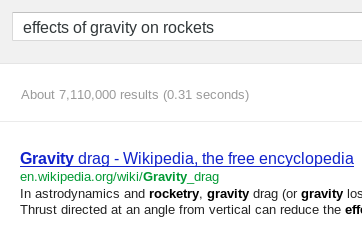
\includegraphics[width=0.80\textwidth]{images/space_rocket_query.png}
\caption{{Google showing over 7M results for ``effects of gravity on rockets"}}
\label{fig:rocket_results}
\end{figure}

Partridge offers an advantage over these mechanisms as it will specifically
index research papers rather than attempting to index the whole Internet.
This means that there should be a higher proportion of useful information as
output compared to the output of an Internet Search Engine.

There are also a number of search and indexing systems that specifically look
for scientific papers as opposed to web pages. One of the most publicised and
well known paper search system is Google Scholar
(\url{http://scholar.google.com}).  As can be seen in Figure
\ref{fig:scholar_basic}, This is an adaptation of Google's general search
engine (discussed above) to specifically index and search scientific papers.
Google also offers advanced query options specific to Scholar that allow
searching by author, year and for words that occur only in the document title
as shown in figure \ref{fig:scholar_advanced}. Whilst this does deal with the
problem of `information overload' and provides even more fine control over the
information returned from searches,  the user is still required to have a very
good idea of what they are looking for in terms of keywords and/or specific
authors. It is possible that a user would not know what they are looking for
until they've seen it. Even if the user has a set of keywords to search for,
they can only search the title of the paper or the content as a whole. This
means that users who want to find a particular phrase within a CoreSC part of
the paper (e.g. only look for this phrase in the `Result' section of the
paper) are unable to get results at their desired level of detail.

\begin{figure}[!hbt]
        \centering
        \begin{subfigure}[b]{0.50\textwidth}
                \centering
                
\includegraphics[width=\textwidth]{images/googlescholar_front.png}
                \caption{Google Scholar's General front page}
                \label{fig:scholar_basic}
        \end{subfigure}%
        \begin{subfigure}[b]{0.50\textwidth}
                \centering
                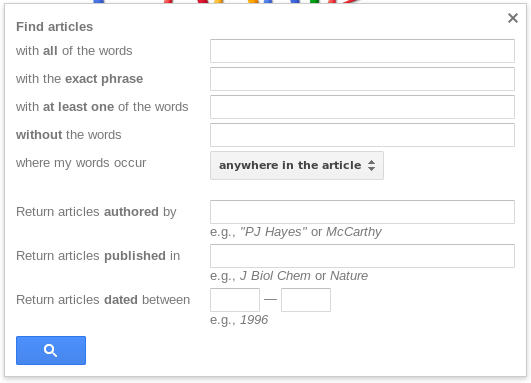
\includegraphics[width=\textwidth]{images/googlescholar_advanced.png}
                \caption{Advanced search features}
                \label{fig:scholar_advanced}
        \end{subfigure}

        \caption{Google Scholar's user interface}
        \label{fig:scholar_interface}
\end{figure}

Partridge will provide the option to filter papers by subject and it is hoped
that the system will also provide user-specific recommendations by profiling
them through their reading history. This will make it easier for users to find
relevant papers without knowing exactly which keywords they need to search for.
Partridge will also offer facilitate searching for keywords within a specific
CoreSC section by making use of Liaketa et al's SAPIENTA project for
classifying each sentence of paper. 


\subsection{Methodology}

\subsection{Prototyping/Pilot Studies}

\subsection{Subsequent Changes to Methodology}

\section{Planning}

\pagebreak
\bibliographystyle{IEEEannot}
\bibliography{report}

\end{document}
